\section{Message Passing Algorithms on Trees}

If the factor graph is a tree, many problems can be solved efficiently using a form of dynamic programming called \emph{message passing}. \newline 
In general, message passing algorithms compute values for each edge of the factor graph. These values can be interpreted as \emph{messages} that are sent between the nodes. Since all edges connect factor nodes to variable nodes there can be two types of messages: messages passed from a variable $i$ to a factor $a$, denoted as $\mu_{i \rightarrow a}$ and messages passed from $a$ to $i$, denoted as $\mu_{a \rightarrow i}$. \newline
The messages must be defined so that a message $\mu_{a \rightarrow i}$ is determined by the messages $\mu_{j \rightarrow a}$ that $a$ received from neighbour variables $j \neq i$. 
The same must hold for $\mu_{i \rightarrow a}$. \newline
Usually the massages $\mu_{i \rightarrow a}$ are obtained by summing over $\mu_{b \rightarrow i}$ and $\mu_{a \rightarrow i}$ by multiplying the messages $\mu_{j \rightarrow a}$. The fundamental equation often has the form \textbf{TODO} $$\mu_{a \rightarrow i} = \prod_{j \in V(a) \setminus i} \underbrace{\sum_{b \in V(j) \setminus a} \mu_{b \rightarrow j}}_{\mu_{j \rightarrow a}}$$ Therefore these types of algorithms are called \emph{sum-product}-algorithms. The messages sent from factors to variables only appear as intermediate results in the computation of messages sent from variables to factors. \newline
For tree factor graphs which do not contain cycles the value of $\mu_{i \rightarrow a}$ does not influence its predecessors $\mu_{b \rightarrow i}$. The messages can be computed sequentially starting with the factor graph's leaves.


\section{Message Passing on general graphs}
If a graph contains cycles, the above described messages are in general not well-defined. However, message passing algorithms which are correct for trees can be used as a heuristic for general graphs. \newline
This \emph{loopy} form of message passing consists of two parts. In the initialization  step each message is provisionally assigned a random value. Now that each message is set the sum-product equation can be used not to compute the absolute result but to repeatedly update the provisional values. In each update step the update rule is applied to all edges $a \rightarrow i$. There are several variants how to schedule these update tasks. For example the messages could be updated in parallel (\emph{synchronous}) or step by step (\emph{asynchronous}) in a fixed order. Here, the order of updates is chosen uniformly at random in each update step. If a message changed its value in the beginning of the step the following updates can instantly access and use its new value. 

The goal is to reach a point where no message would significantly change when applying the update rule to it. If this is the case, the messages are said to have \emph{converged}. A point of convergence is also called a \emph{fixed point}. Wether a fixed point is found  does not only depend on the input graph but also on the chosen starting values and the update schedule. Since there is no guarantee that the messages will converge it is possible for the update process to never terminate. In this case the computation has to be terminated after a fixed number of steps. Also an instance can have multiple fixed points that are not the desired solution. The converged messages are therefore only a heuristic solution if the factor graph contains cycles.

For SAT problems experimental results imply that the possibility of convergence is connected to the \textbf{TODO}

On trees this heuristic approach always converges to a unique set of fixed point warnings. The convergence for trees, like other properties of message passing algorithms, can be shown by induction on the \textit{level} of a message.

\begin{wrapfigure}{r}{0.3\textwidth}

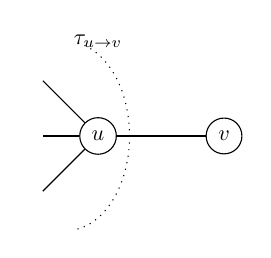
\begin{tikzpicture}[scale=0.8,transform shape]
   	
	\node[shape=circle,draw=black] (u) at (0,0) {$u$};   	
	\node[shape=circle,draw=black] (v) at (2,0) {$v$};  
   	
  
	\node[] (x1) at (-1,0) {};
	\node[] (x2) at (-1,1) {};
	\node[] (x3) at (-1,-1) {};

    \draw[-] (u) edge [right] node {} (x1);
    \draw[-] (u) edge [right] node {} (x2);
    \draw[-] (u) edge [right] node {} (x3);
	
\tikzset{
    partial ellipse/.style args={#1:#2:#3}{
        insert path={+ (#1:#3) arc (#1:#2:#3)}
    }
}	
	
	\draw[-] (u) edge [right] node {} (v);
	\draw[dotted] (-0.5,0) [partial ellipse=-80:80:1cm and 1.5cm];
	\node[] (anon) at (0, 1.5) {$\tau_{u \rightarrow v}$};

\end{tikzpicture}
\end{wrapfigure}
\begin{definition} Let $(u, v)$ be an edge of a tree $\tau$. \newline
The tree $\tau_{u \rightarrow v}$ is the component of $\tau \setminus (u, v)$ that still contains $u$. The \emph{level} of the directed edge $u \rightarrow v$ is the height of $u$ in $\tau_{u \rightarrow v}$. 
\end{definition}
The level can be thought as the length of the longest path in $\tau$ that ends in $u$ and does not pass $v$.
\begin{lemma}\cite{survprob}
On a tree factor graph the message on an edge $a \rightarrow i$ at level $r$ converges after at most $r/2 + 1$ update steps.
\begin{proof} Induction on $r$:
\begin{itemize}
\item[] If $r = 0$, $a$ is a leaf since there are no ingoing messages $j \rightarrow a$ so its message is constant at every step. \newline
Similarly for $r = 1$ all ingoing edges have level $0$ and $m_{a \rightarrow i}$ is constant from step $0$.
\item[] If $r \geq 2$ the message $m_{a \rightarrow i}$ is determined by the set of messages $m_{b \rightarrow j}$ sent to adjacent variables $j$. These messages are sent on edges with level $\leq r-2$ and have by induction converged on step $\frac{r-2}{2} + 1 = r / 2$. $m_{a \rightarrow i}$ converges in the next update step.
\end{itemize}
\end{proof}
\end{lemma}

\begin{figure}[h]
\centering

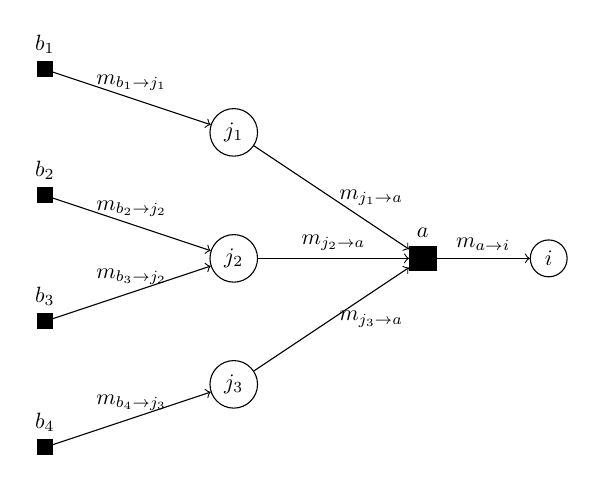
\begin{tikzpicture}[scale=0.8,transform shape]
   	\node[rectangle,draw=black, label = {$a$}, fill] (i) at (3,0) {$a$};
    \node[shape=circle,draw=black] (a) at (5,0) {$i$};
   
  \node[shape=circle,draw=black] (b1) at (0,2) {$j_1$};
  \node[shape=circle,draw=black] (b2) at (0,0) {$j_2$};
  \node[shape=circle,draw=black] (b3) at (0,-2) {$j_3$};

	\node[rectangle,draw=black, label = {$b_1$}, fill] (j1) at (-3,3) {};
	\node[rectangle,draw=black, label = {$b_2$}, fill] (j2) at (-3,1) {};
	\node[rectangle,draw=black, label = {$b_3$}, fill] (j3) at (-3,-1) {};
	\node[rectangle,draw=black, label = {$b_4$}, fill] (j4) at (-3,-3) {};


    
	\draw[->] (b3) edge [right] node {$m_{j_3 \rightarrow a}$} (i);
	\draw[->] (b2) edge [above] node {$m_{j_2 \rightarrow a}$} (i);
	\draw[->] (b1) edge [right] node {$m_{j_1 \rightarrow a}$} (i);
	\draw[->] (i) edge [above] node {$m_{a \rightarrow i}$} (a);
	
	\draw[->] (j1) edge [above] node {$m_{b_1 \rightarrow j_1}$} (b1);
  	\draw[->] (j2) edge [above] node {$m_{b_2 \rightarrow j_2}$} (b2);
	\draw[->] (j3) edge [above] node {$m_{b_3 \rightarrow j_2}$} (b2);
	\draw[->] (j4) edge [above] node {$m_{b_4 \rightarrow j_3}$} (b3);

\end{tikzpicture}
\caption{Subgraph of a factor tree with all messages required for computing $m_{a \rightarrow i}$}
\end{figure}